\chapter{Resultados}\label{cap:resultados}
		\subsection{Quadro Comparativo}
	
	% Please add the following required packages to your document preamble:
	% \usepackage[table,xcdraw]{xcolor}
	% If you use beamer only pass "xcolor=table" option, i.e. \documentclass[xcolor=table]{beamer}
	% \usepackage{lscape}
	\begin{landscape}
		\begin{table}[H]
			\centering
			\caption{Tabela Comparativa entre Bibliotecas de Realidade Aumentada}
			\label{tabComparativa}
			\begin{tabular}{|l|c|c|c|c|}
				\hline
				& \multicolumn{1}{l|}{\cellcolor[HTML]{FFFC9E}\textbf{ARToolKit}} & \multicolumn{1}{l|}{\cellcolor[HTML]{FFFC9E}\textbf{Vuforia}} & \multicolumn{1}{l|}{\cellcolor[HTML]{FFFC9E}\textbf{Layar}} & \multicolumn{1}{l|}{\cellcolor[HTML]{FFFC9E}\textbf{ARCore}} \\ \hline
				\cellcolor[HTML]{FFFC9E}\textbf{Custo} & Grátis & \begin{tabular}[c]{@{}c@{}}Desenvolvimento Grátis, \\ Implantação \$499 ou\\ \$99 por Mês\end{tabular} & \begin{tabular}[c]{@{}c@{}}\$15.99 Por Página ou\\  \$79 Por Página\end{tabular} & Grátis \\ \hline
				\cellcolor[HTML]{FFFC9E}\textbf{Plataforma desenvolvimento} & \textbf{\begin{tabular}[c]{@{}c@{}}Unity,\\ Android Stúdio,\\ Unreal\end{tabular}} & \begin{tabular}[c]{@{}c@{}}Unity, \\ Android Studio, \\ XCode, \\ Vuforia Studio\end{tabular} & Layar Studio & \begin{tabular}[c]{@{}c@{}}Unreal,\\  unity,  \\ Android Studio, \\ XCode\end{tabular} \\ \hline
				\cellcolor[HTML]{FFFC9E}\textbf{\begin{tabular}[c]{@{}l@{}}Plataforma\\ execução\end{tabular}} & \begin{tabular}[c]{@{}c@{}}PC, \\ Android, \\ iOs\end{tabular} & \begin{tabular}[c]{@{}c@{}}PC, \\ Android, \\ iOs\end{tabular} & PC, Android, iOs, Blackbarry & \begin{tabular}[c]{@{}c@{}}Android, \\ iOs\end{tabular} \\ \hline
				\cellcolor[HTML]{FFFC9E}\textbf{Documentação} & \begin{tabular}[c]{@{}c@{}}http://www.hitl.\\ washington.edu/\\ artoolkit/\\ documentation/\end{tabular} & \begin{tabular}[c]{@{}c@{}}https://library.\\ vuforia.com/\\ getting-started/\\ overview.html\end{tabular} & \begin{tabular}[c]{@{}c@{}}https://www.layar.com\\ /documentation/browser/api/\end{tabular} & \begin{tabular}[c]{@{}c@{}}https://developers.\\ google.com/ar/\\ reference/\end{tabular} \\ \hline
				\cellcolor[HTML]{FFFC9E}\textbf{Linguagem} & \begin{tabular}[c]{@{}c@{}}C/C++, \\ Java,\\ C\#\end{tabular} & \begin{tabular}[c]{@{}c@{}}C++,\\ Java e\\ .Net\end{tabular} & JavaScript & Java, C\# , C++ \\ \hline
			\end{tabular}
		\end{table}
	\end{landscape}
	
Ao se realizar o estudo das bibliotecas de realidade aumentada e as por em um quadro comparativo como é mostrado na tabela \ref{tabComparativa}, pode ser visto que a biblioteca ARCore lançada pela google tem atributos importantes para o desenvolvimento desse trabalho, como o fato de a mesma ser grátis e ter ajudas e exemplos disponibilizados pela própria google no github, a gama de ambientes de desenvolvimento é bem ampla, e tendo assim também uma quantidade de linguagens de programação que pode ser usada.

Um ponto que deve ser levado bastante em consideração para um desenvolvedor é a documentação que a tecnologia usada disponibiliza, e a ARCore tem uma documentação bastante extensa e explicativa, e abrangendo todos os ambientes de desenvolvimento.

A Biblioteca ARCore apesar de ser da google e ser especifica para a plataforma Android possui uma compatibilidade com a biblioteca de Realidade aumentada da \textit{Apple}, a ARKit, fazendo assim com que o desenvolvimento de aplicativos nesta plataforma possa ser traduzido para ARKit.

Por fim, como será usado a ferramenta de mapas \textit{Google Maps}, a integração com a biblioteca de AR será feita de maneira mais fluida pelo fato de as duas bibliotecas serem mantidas e desenvolvidas pela mesma empresa, Google.

\section{Trabalhos Futuros}
Como trabalhos futuros poderá ser desenvolvidas uma biblioteca que irá fazer o uso da realidade aumentada por meio da biblioteca \textit{ARCore By Google}, que foi uma das estudadas por este trabalho, sendo feita em conjunto com geolocalização, usando as biblioteca \textit{Google Maps}, na qual por meio desta API poderá ser desenvolvidas aplicações que usem esses dois recursos.
 
Para demonstração será desenvolvido um aplicativo que ira servir de guia turístico,usando Realidade aumenta e Geolocalização ele irá mostrar informações em locais destinados ao turismo, estes dados deverão ser cadastrados para cada localização baseando-se em latitude e longitude, desta maneira, o turista poderá ter uma experiência mais profunda naquele local.

\begin{figure}[H]
	\centering
	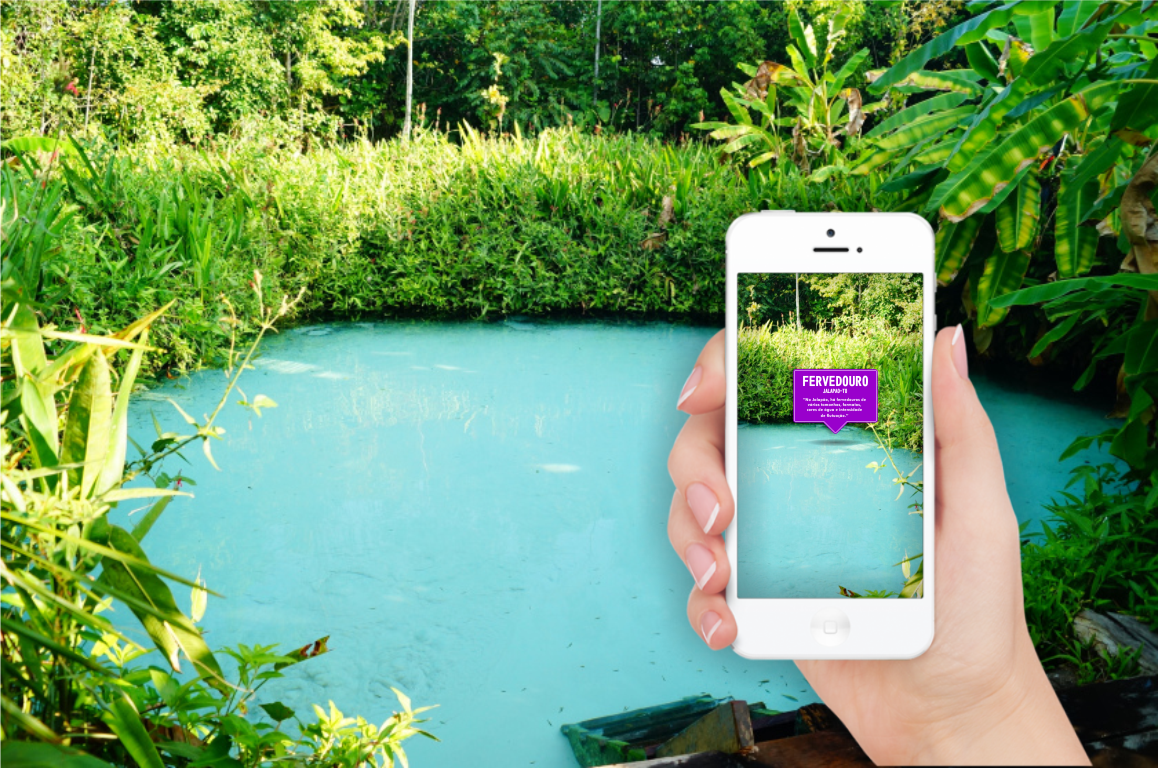
\includegraphics[scale=1.1]{imagens/fervedouro}
	\caption{Exemplo de Funcionamento do ARTur}
	Fonte: Autor, 2018
	\label{fig:artur}
\end{figure}

A Figura \ref{fig:artur} é uma demonstração de como deverá ser o aplicativo, onde o turista/usuário ira apontar a câmera de seu celular para um determinado ponto turístico que tenha sua geolocalização previamente cadastrada e aparecerá uma placa virtual sobrepondo-se a imagem do mundo real, sendo que com isso ele poderá interagir com aquela figura virtual.

\begin{figure}[H]
	\centering
	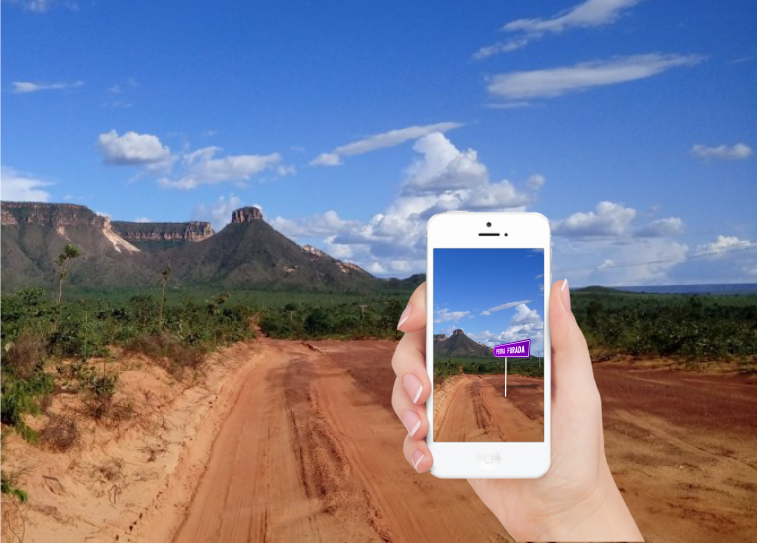
\includegraphics[scale=1.5]{imagens/estrada}
	\caption{Exemplo de Funcionamento do ARTur com Setas Indicativas}
	Fonte: Autor, 2018
	\label{fig:artur2}
\end{figure}

A Figura \ref{fig:artur2}, se trata de outro exemplo de como será a aplicação desenvolvida a partir da biblioteca gerada, onde poderão ser colocadas também placas indicativas que ajudará os turistas a encontrar locais turísticos que eles desejam chegar.
%-------------------------------------------------------------------------------------
%	- TCC
%	- Montagem da arquitetura para o desenvolvimento de apps
%	baseadas em RA e geolocalização	
%-------------------------------------------------------------------------------------